\chapter{Restos de ABC}\label{apendix:restosDeABC}

%%%%%%%%%%%%%%%%%%%%%%%%%%%%%%%%%%%% SISTEMAS ABC:TRAZABILIDAD %%%%%%%%%%%%%%%%%%%%%%
\section{Trazabilidad}\label{sec:Trazabilidad}

Para posteriormente analizar y realizar controles de calidad, toda la información generada por los sistemas \GLS{ABC} debe ser almacenada de forma estructurada (bases de datos, o ficheros XML) y anónima, sin indicar la identidad del viajero. 

La información referente a los accesos y a la monitorización en general debe almacenarse de forma centralizada a nivel instalación. Mientras que la información de las operaciones y la traza de la aplicación es conveniente guardarla a nivel local.

Es recomendable guardar la mayor cantidad de información posible por cada cruce.
\begin{enumerate}
    \item 
    Viajeros con documentos no aceptados, documentos no \GLS{MRTD} o pasaportes abiertos por una página distinta a la de datos.
    \item 
    Viajeros con documentos válidos pero no elegibles, por su nacionalidad o por no cumplir los requerimientos del país.
    \item 
    Viajeros elegibles, con documentos aceptados pero que no han conseguido ser verificados en la verificación biométrica.   
\end{enumerate}


%%%%%%%%%%% SISTEMAS ABC:PROTECCION DE DATOS %%%%%%%%%%%%%%%%%%%%%%
\section{Protección de datos}\label{sec:ProtecionDatosABC}

\color{magenta} CRISTINA: Ampliarlo y meter algo del RGPD y de la LOPDGDD \color{black}

\color{cyan}
Los sistemas deben atender a las leyes de protección de datos de cada país y deben tener en cuenta ésta protección tanto en su diseño como en su implementación.

En el caso de Europa \cite{EUOnline} las leyes de protección de datos viene definida en:

Europe Data protection regulation $2012$ General data protección regulation.

Articulo 8 de la convención de derechos humanos Europea.

European Data Protection Supervisor
\color{black}

\begin{figure}[t]
    \centering
    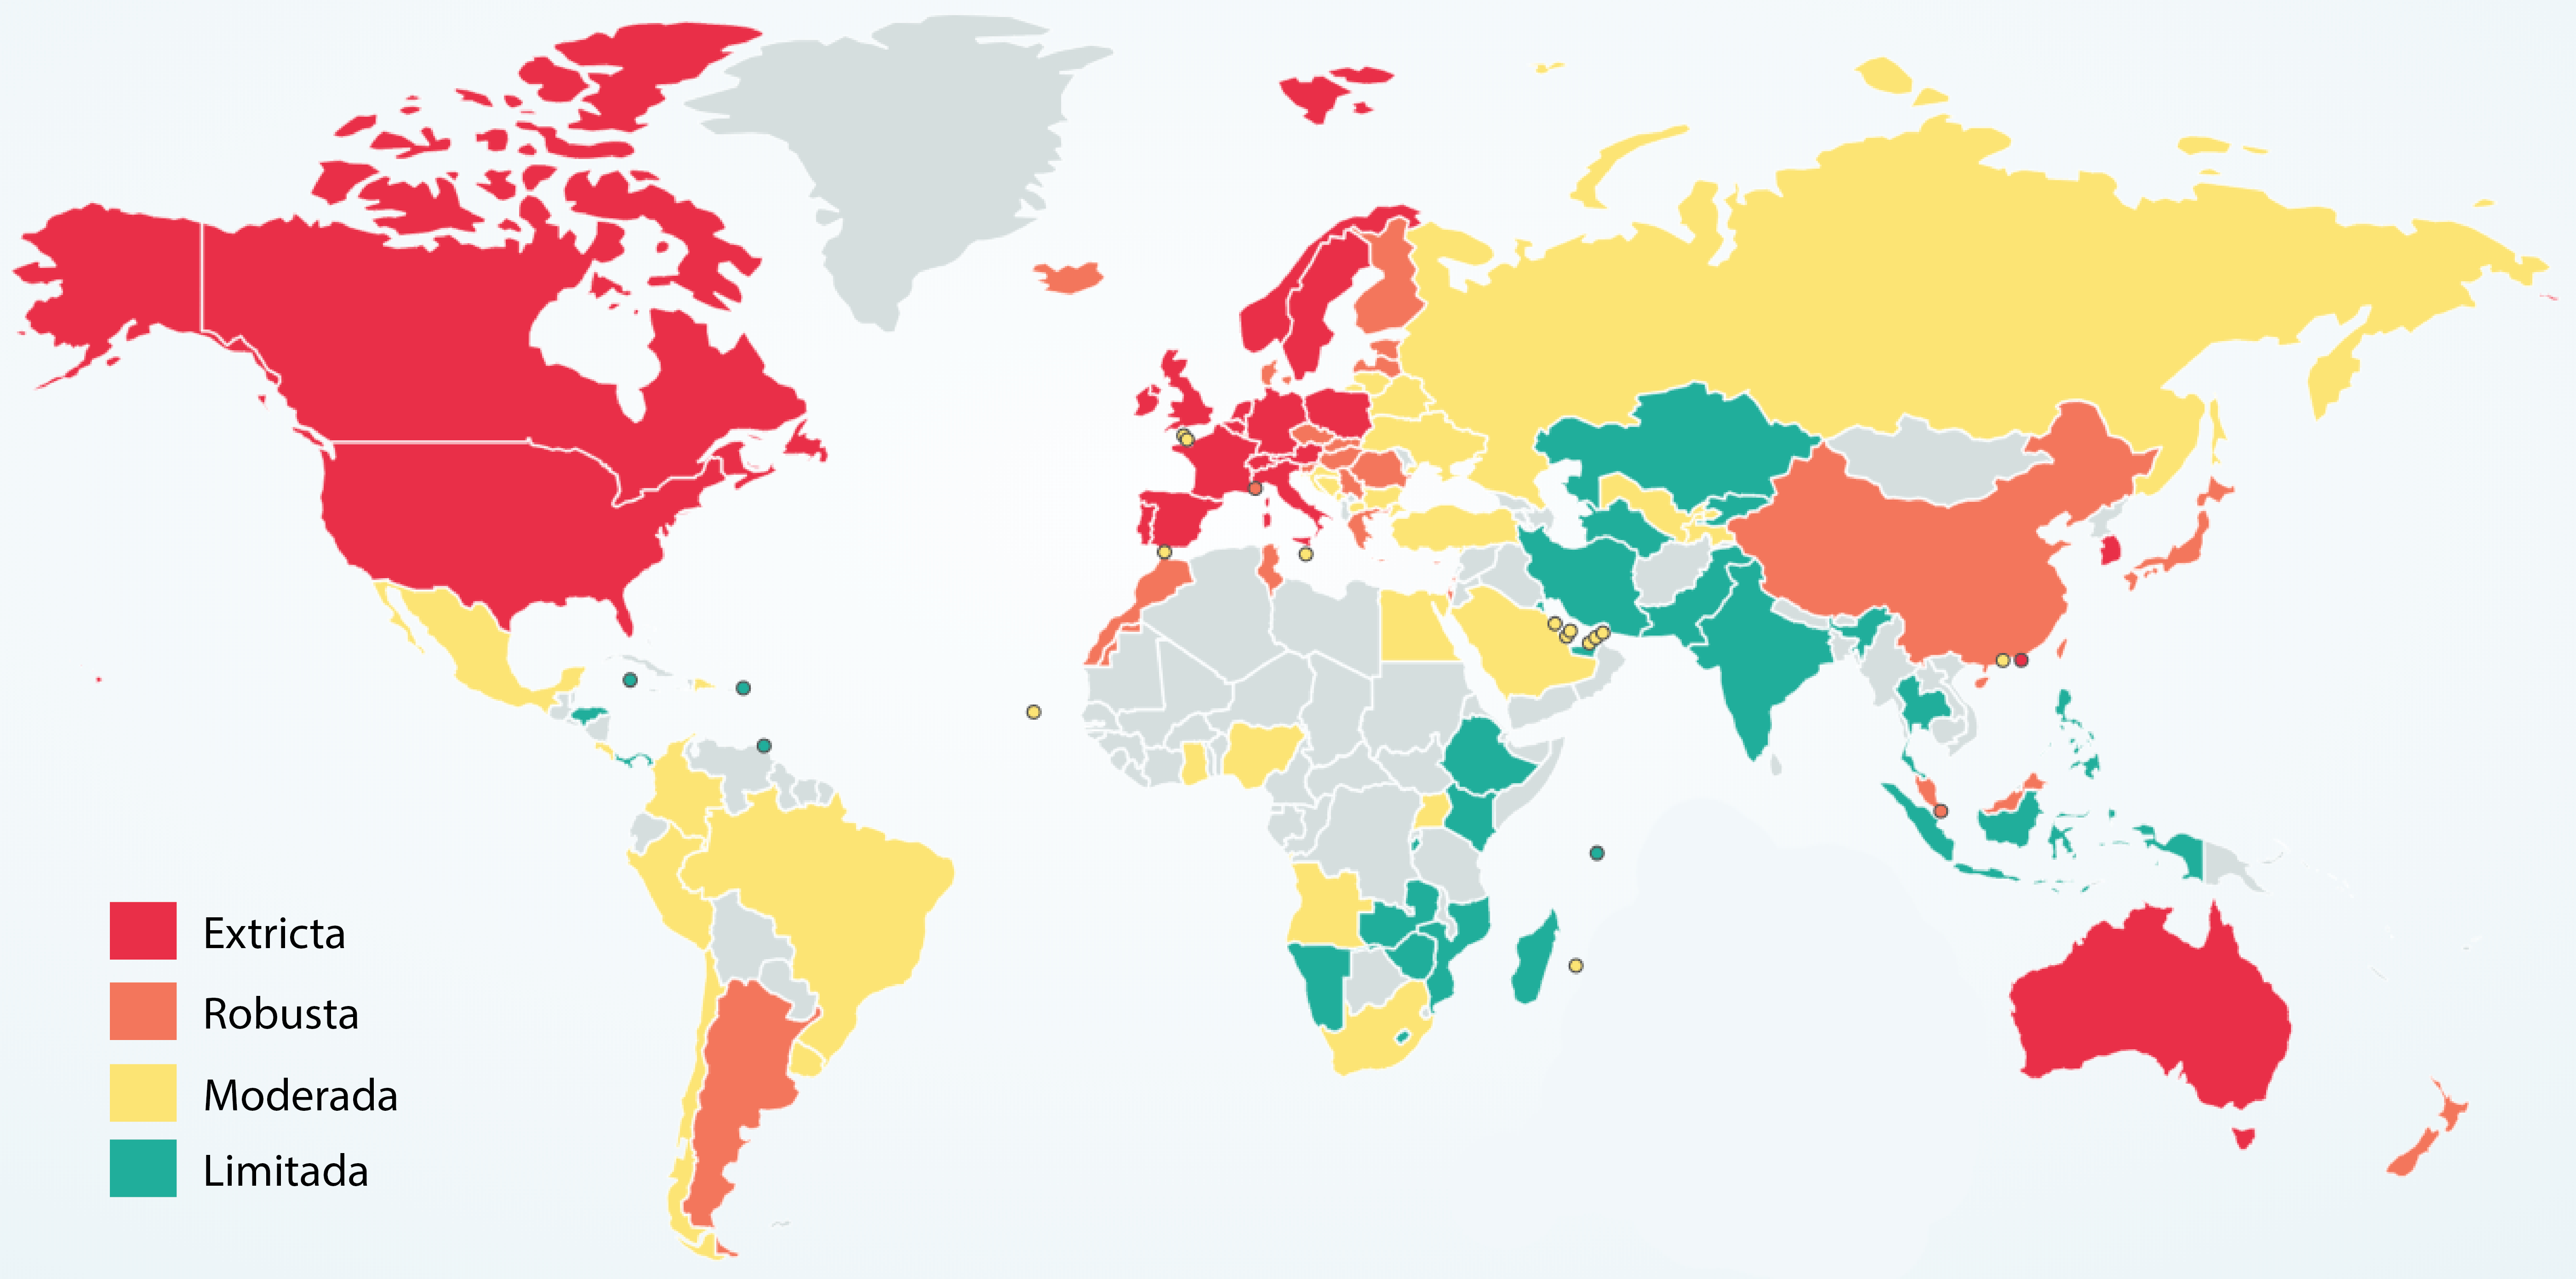
\includegraphics[width=0.9\textwidth]{ch-sistemasABC/images/ch-SistemasABC/proteccionDatosPaises.png}
    \caption{Leyes de protección de datos en el mundo \cite{DLAPiperOnline}.}
    \label{fig:mapaLeyesProteccionDatos}
\end{figure}


%%%%%%%%%%%%%%%%%%%%%%%%%%%%%%%%%%%% SISTEMAS ABC:PERSONAL HUMANO %%%%%%%%%%%%%%%%%%%%%%
\section{Personal humano en los sistemas ABC.}\label{sec:PersonalABC}

Existen dos roles necesarios en el trabajo con los sistemas \GLS{ABC}: Operadores y asistentes.

\paragraph{Operadores\\}

Se encargan de la monitorización del sistema.

\begin{itemize}
    \item
    Monitorizan los sistemas.
    \item
    Atender las incidencias y decidir sobre ellas.
    \item
    Vigilar el orden de la cola de espera.
    \item
    Controlar si los viajeros que están esperando cumplen los requisitos para acceder, por nacionalidad o por edad.
    \item
    Detectar a los viajeros sospechosos que requieran un control más exhaustivo. Por su vestimenta o por su comportamiento.
\end{itemize}

\paragraph{Asistentes\\}

Son los guardias de seguridad del control de fronteras.

\begin{itemize}
    \item 
    Ayudan a los operadores en el manejo de las excepciones y en la detección de pasajeros sospechosos.
    \item
    Redirigir a los pasajeros a los controles manuales si es necesario.
    \item
    Informar y ayudar a los viajeros
    \item
    Asistir a las personas con problemas para el manejo de los sistemas.
\end{itemize}
    
El número de dispositivos \GLS{ABC} a instalar también depende del número de agentes disponibles. Cada agente de seguridad puede vigilar aproximadamente de $3$ a $10$ sistemas \GLS{ABC} \cite{FRONTEX2016OpeReport}. Dependiendo de distintos factores como:

\begin{itemize}
    \item 
    La calidad del sistema biométrico, la fiabilidad de los reconocedores faciales y de las huellas. Y también del sistema de detección de ataques de suplantación de identidad.
    \item
    De la frecuencia de pasajeros.
    \item
    De la disposición de los dispositivos si están en la salida o en la entrada de la frontera.
    \item
    Del perfil de los pasajeros. Si es la primera vez que usan el sistema o ya lo han usado antes.
    \item
    Del diseño del interfaz, si es o más o menos fácil de usar.
    \item
    De la formación o de la capacitación de los agentes de seguridad.
\end{itemize}

Con el tiempo el número de agentes puede ajustarse atendiendo a las necesidades. 

 
 
%%%%%%%%%%%%%%%%%%%%%%%%%%%%%%%%%%%% SISTEMAS ABC:METRICAS Y EVALUACION %%%%%%%%%%%%%%%%%%%%%%
\section{Métricas y Evaluación??}
\color{cyan} aquí seran los rechazos mas que los errores biométricos\color{black}

Métricas como \GLS{FAR} o \GLS{FRR} miden el aspecto técnico del sistema pero no tienen en cuenta el factor humano o la experiencia de usuario de los viajeros \cite{el2010study}. Si la primera experiencia de un viajero con el sistema es mala, no volverá a usarlo \cite{macleod2011methodology} \cite{graves2011role}.

Que muchos usuarios hagan uso de los sistemas \GLS{ABC} no garantiza que el proceso del cruce de fronteras sea más eficiente, incluso podría ser contraproducente. Hasta que los usuarios no aprenden el manejo del sistema no habrá optimización alguna. Por lo que es importante tener en cuenta la experiencia de usuario y la curva de aprendizaje del sistema.   

Existen casos en que los viajeros son reticentes a usar los sistemas ABC. Es posible distinguir los siguientes tipos de viajero reticentes \cite{oostveen2014non}:

\begin{itemize}
    \item 
    \textbf{Resistentes}: Aquellos viajeros que se niegan directamente a usar la tecnología.
    \item
    \textbf{Rechazadores}: Antiguos usuarios del sistema que por alguna mala experiencia no quieren volver a usarlo.
    \item
    \textbf{Excluidos}: Usuarios que quieran o no usar el sistema, no pueden por limitaciones físicas o intelectuales.
    \item
    \textbf{Expulsados}; Usuarios que no cumplen los requisitos para usar el sistema.
    \item
    \textbf{Desconocedores}: Los viajero que directamente no saben que existe.
\end{itemize}

Desde el punto de vista de la \gls{usabilidad} se deben tener en cuenta aquellos factores que influyan en el acceso al sistema de viajeros con características especiales;. Por ejemplo personas con alguna discapacidad, movilidad reducida o personas de edad avanzada\cite{sasse2013usable}.



%%%%%%%%%%%%%%%%%%%%%%%%%%%%%%%%%%%% SISTEMAS ABC:VENTAJAS DEL USO DE LOS ABC %%%%%%%%%%%%%%%%%%%%%%
\section{Ventajas}\label{sec:VentajasABC}

Facilita el proceso de los viajero y maximiza la seguridad.

Incrementar el número de viajero sin necesidad de incrementar el numero de agente de control.

El proceso automatizado de los \GLS{ABC} ofrece una serie de ventajas:

\begin{itemize}
     \item
     Identificación de grandes grupos de personas.
      \item
      Reducir los tiempos de de transito.
      \item
      Reducir el tamaño de los dispositivos para instalaciones reducidas.
      \item
      Mejorar la \gls{usabilidad}.
      \item
      Reducir los costos de los dispositivos y las instalaciones.
      \item
      El incremento del número de viajeros.
\end{itemize}

\begin{itemize}
    \item 
    Comparado con el proceso manual se reducen considerablemente los tiempos de espera y se acelera el flujo de viajeros.
    \item 
    Incrementa la seguridad ya que se incluye la validación biométrica de los datos almacenados en el \gls{eMRTD}. De forma que es posible detectar falsificaciones e impostores.
    \item
    Disminuye la carga de trabajo de los agentes fronterizos, además de que un único agente puede controlar varias puertas.
    \item
    Mejora la experiencia del viajero.
\end{itemize}

En algunos tipos de fronteras Las ventajas que pueden ofrecer los \GLS{ABC} son aun mayores. Por ejemplo para trasportes como trenes o autobuses en fronteras terrestres o cruceros en fronteras marítimas, donde no seria necesario el desembarco de los viajeros.

A la par que avanza la tecnología se incrementan las ventajas que ofrecen los \GLS{ABC}.

Algunos \GLS{ABC} utilizan la biometría del \gls{iris} para la identificación. Esta biométrica se basa en el patrón muscular de esta parte del ojo y se suele leer con cámaras \gls{IR}. Se trata de una biometría poco intrusiva y con una alta aceptación por parte de ciertas culturas.

El uso de lectores de huellas dactilares sin contacto supone una importante mejora ya que se tienen mayor aceptación que los lectores actuales que se consideran menos higiénicos.


%%%%%%%%%%%%%%%%%%%%%%%%%%%%%%%%%%%% SISTEMAS ABC:RETOS DE ABC %%%%%%%%%%%%%%%%%%%%%%%%%%%%%%%%%%%5
\section{Retos}\label{sec:RetosABC}

Desde el punto de vista del sistema biométrico los retos con los que se enfrentan los \GLS{ABC} son:
\begin{itemize}
    \item
    Buscar rasgos biométricos menos intrusivos: 
    
    Huellas dactilares sin contacto\cite{labati2015touchless} \cite{labati2015toward}, palma de la mano sin contacto, \cite{genovese2014touchless}, iris a distancia \cite{matey2006iris}.
    
    \item
    Verificación en condiciones menos controladas:
    
    Iluminación natural, grandes distancias, \gls{captura} en movimiento
    
    \item
    \Gls{captura} sin contacto (\textit{\gls{contactless}} o \textit{\gls{touchless}})
    
    \item
    Dispositivos de adquisición apropiados para los retos planteados:
    
    Escáneres y cámaras de alta resolución, sensores multiespectrales, software dedicado. 
    
    Dispositivos móviles que faciliten la accesibilidad \cite{FastPassOnline}.
    
    \item
    Software dedicado y algoritmos adaptados \cite{abiantun2014sparse}.

\end{itemize}

\color{red}NFC??\color{black}


%%%%%%%%%%%%%%%%%%%%%%%%%%%%%%%%%%%% SISTEMAS ABC:ERGONOMIA %%%%%%%%%%%%%%%%%%%%%%
\section{Requisitos de los sistemas ABC: ergonomía y usabilidad}\label{sec:ErgonomiaABC}

\color{red}

Siempre debe haber un agente de seguridad controlando los sistemas automáticos y debe estar capacitado para dar respuesta ante cualquier tipo de fallos.

El numero de sistemas dependerá del número de viajeros y del numero de agentes disponibles para controlarlos. La configuración de los sistemas debe ser flexible para que sea posible activar o desactivar algunos sistemas dependiendo del flujo de viajeros en un momento dado.

Los sistemas \GLS{ABC} deben de ser intuitivos y fáciles de manejar por los viajeros.

No debe ser posible esquivar el control.

Controlar que no crucen menores.

Deben existir procedimientos de contingencia para todos los posibles problemas.

Seleccionar la mejor pose atendiendo a dos factores de calidad:
\begin{itemize}
     \item
     Factores de la imagen: Nitidez. contraste, artefactos.
     \item
     Factores de la cara: Pose, expresiones, sombras, oclusiones (gorros, gafas, etc.)
\end{itemize}

\color{black}

\color{red}ESTO ES PARA COLOCAR Y VERIFICAR SI NO ESTA DUPLICADO

Los dispositivos deben ser compactos para evitar que los sensores o los componentes periféricos sean manipulados por los viajeros.

Deben ser robustos para que una personas sin acceso no puedan derribarlos, pasar por encima de las barreras o por debajo.

Modulares para poder modificar o reemplazar componentes aislados sin tener que afecte al resto del sistema.

Evitar anclajes fijos, para poder cambiar la distribución de los sistemas en el área del cruce de frontera, si resulta necesario. 

Estar cerca de la primera linea para que los agentes puedan atender las incidencias y para que el viajero pueda ser redirigido al control manual en caso de fallo.

Tener en cuenta el tamaño de los equipaje y las necesidades especiales que puedan tener alguno viajeros.
\color{black}


La usabilidad de los sistemas \GLS{ABC} debe considerar aspectos de ergonomía de los dispositivos que intervienen en el sistemas (dispositivos de adquisición, sensores, \textit{interfaces}, \textit{displays}, etc.) y otros aspectos relacionados con la señalización, las indicaciones o las ayudas al viajero. 

Los procesos a realizar en el sistema deben tener una secuencia lógica 

Debe prestar especial atención a las personas discapacitadas.

Debe ser flexible para adaptarse y hacer frente a las posibles incidencias.

Los estándares definidos en \GLS{CEN}/TS 16634:2014 \cite{CEN/TS16634:2014}, ISO \cite{ISO/Biometric} y \Gls{frontex} \cite{FRONTEX2016OpeReport} \cite{FRONTEX2016TechReport} recomiendan las siguientes medidas para mejorar la usabilidad y la \gls{ergonomia} de los sistemas \GLS{ABC}:

\begin{itemize}
    \item
    El sistema debe usarse con el mínimo esfuerzo posible. Minimizar las interacciones con sistema y reducir número de veces que el usuario tiene que usar las manos para evitar que el viajero tenga que estar dejando o cambiando de mano su equipaje. 
    \item
    Adecuar la altura de adquisición de lectores del pasaporte y del resto de sensores deben estar a una altura adecuada para la mayoría de las personas.
\end{itemize}

Los estándares también proponen una serie de consejos a tener en cuenta sobre la información que debe ser suministrada al viajero y el formato que ésta debería tener.

\begin{itemize}
    \item
    Indicar con la mayor antelación posible los requisitos que debe cumplir el viajero para usar el sistema. Indicar que viajeros pueden usar o no, el sistema.  
    \item
    Informar de forma anticipada del estado del sistema. No sólo si se encuentra disponible si no también de los tiempos estimados de espera y de proceso.
    \item
    Toda las instrucciones que se suministren al viajero deben de ser intuitivas, inequívocas y autoesplicativas.
    \item
    La información debe proporcionarse en distintos formatos: visuales, audibles y simbólicas. Se recomiendan señales parpadeantes que atraigan la atención del viajero.
    Una buena práctica es guiar la atención del viajero en los distintos pasos del proceso a realzar, activando y desactivando una señal luminosa o sonora en el elemento del dispositivo con el que debe interactuar en cada momento. Por ejemplo, escáner de documento, escáner dactilar, cámara para la captura \gls{facial}, etc.
    \item
    Información en distintos idiomas que el viajero pueda entender.
    \item
    Que todos los fabricantes de dispositivos \GLS{ABC} usen los mismos símbolos\footnote{ISO/\GLS{IEC} JTC1 SC37 \textit{in project} 24779 \cite{ISO/Biometric} propone un estándar para la mayoría de los símbolos usados en la  señalización de los sistemas \GLS{ABC}.} para su señalización facilita la ejecución de los procesos, al viajero.
    \item
    El sistema debe dar un \textit{feedback} continuo al viajero, indicando que proceso se esta realizando en cada momento, especialmente cuando se estén realizando procesos de adquisición, que pueden resultar más lentos. También se debe devolver una respuesta clara para confirmar si los procesos se han realizando correctamente
\end{itemize}

Es también aconsejable realizar una labor de divulgación y de formación previa al viajero.

\begin{itemize}
    \item
    Distribuir folletos, anuncios o vídeos ilustrativos del proceso que enseñen cómo usar el sistema y quienes pueden acceder al él. 
    \item
    Ubicar personal de información cerca de los dispositivos. 
    \item
    Explicar los beneficios que tienen los sistemas automáticos, explicando lo fácil y rápido que resulta usarlos.
\end{itemize}

Es aconsejable que lo sistemas se instalen en una ubicación interior donde las condiciones ambientales están más controladas, pero aun así, cuando es necesaria una instalación en algún lugar público, transitado o en el exterior se deben tener en cuenta aspectos específicos para este tipo de instalaciones.

\begin{itemize}
    \item 
    Condiciones de luminosidad.
    \item
    Condiciones climáticas.
    \item
    Condiciones de contaminación o deterioro.
\end{itemize}
    
Además de tener en cuenta los aspectos técnicos a la hora de realizar la instalación de los sistemas \GLS{ABC}, como la electricidad, las conexiones o el cableado. \Gls{frontex} en \cite{FRONTEX2016OpeReport}, también señala una serie de medidas a tener en cuenta en la infraestructura que tiene más que ver con la usabilidad de los sistemas.

\begin{itemize}
    \item
    Los sistemas \GLS{ABC} deben estar cerca de las controles manuales, para facilitar el paso de unos a otros en caso de que sea necesario y para que los agentes de seguridad puedan asistir rápidamente las incidencias que puedan producirse en lo sistemas automáticos.
    \item
    Los sistemas automáticos deben estar colocados de forma que sean visibles al entrar en el área del cruce de frontera. Normalmente si lo viajeros divisan primero los controles manuales no accederán a los controles automáticos.
    \item
    Los sistemas debe instalarse facilitando el flujo normal de los viajeros y tratando de evitar las aglomeraciones.
    \item
    Es aconsejable que los controles se coloquen en paralelo y de forma que resulte visibles para el resto de viajeros que están esperando. De esta forma, los viajeros pueden ir aprendiendo viendo el uso del sistema mientras esperan.
    
    Cuando los sistemas se colocan en paralelo, conviene analizar previamente, las interferencias que pueden producirse entre unos y otros. Como por ejemplo, interferencias de las señales sonoras o de las fuentes de luz.  
    \item
    Es importante controlar la iluminación de área en la que van a instalarse los sistemas de instalación especialmente para la adquisición \gls{facial}, ya que que una mala iluminación puede alterar el resultado del sistema.
    \item
    El número de sistemas a instalar depende del flujo de viajeros, pero también se debe considerar que cada maquina incrementa los costes de mantenimiento, de control y de monitorización. La calidad del sistema se mide en el tiempo que un sistema tarda por cada viajero. El objetivo debe ser reducir el tiempo por viajero y aumentar el número de viajeros.
    \item
    Los sistemas deben diseñarse de forma modular para que se posible aplicarse fácilmente y adaptarse a las nuevas necesidades y requisitos.
\end{itemize}

Las personas de con alguna discapacidad tienen preferencia para acceder a los controles manuales. Aun así los sistemas automáticos deben tener en cuenta para viajeros con alguna discapacidad.


\begin{itemize}
    \item 
    Verificar que la localización del \GLS{ABC} para que sea accesible a todas las personas.
    \item
    Señalización correcta para acceder al sistema: Guías en el suelo, bandas sonoras y señalización para personas invidentes.
    \item
    Información en distintos formatos (audio, visuales con fuentes grandes y de fáciles de leer).
    \item
    Adaptar los dispositivos para el acceso de sillas de ruedas.
    \item
    Dispositivos de captura colocados a una altura adecuada para personas en sillas de ruedas.
    \item
    Controlar el sistema de cierre de compuertas para personas de edad avanzada con dificultad de movimiento o con movilidad reducida.
    \item
    Instalación de intercomunicadores en los dispositivos que permitan comunicarse con los agentes encargados de la monitorización.
    \item
    tener en cuenta en los interfaces y en la señalización los colores, para viajeros con problemas de percepción cromática (personas con acromatopsia o daltonismo).
    \item
    Agentes especializados en la asistencia a personas con alguna discapacidad.
\end{itemize}

A la hora de diseñar dispositivos \GLS{ABC} también se deber tener en cuenta una serie de factores para la usabilidad y la \gls{ergonomia}. 

\begin{itemize}
    \item 
    Deben diseñarse para que resulten eficientes para los viajero y para los agentes.
    \item
    Debe resultar atractivo para los viajero. Por ejemplo, los dispositivos \textit{\gls{mantrap}} intimidan más a los viajeros que los dispositivos de tipos \textit{\gls{e-kiosk}}. O también, los cristales trasparentes en las barreras, dan más confianza al viajero que los materiales opacos o los cristales ahumados.
    \item
    Tener en cuenta el tamaño del equipaje de los viajeros y facilitar la movilidad en el dispositivo.
\end{itemize}

En las sección sec:ErgonomiaBiometricosABC se proponen otras medias para mejorar la ergonomía y la usabilidad de los sistemas \GLS{ABC}, especialmente en aspectos que afectan al sistema biométrico.


%%%%%%%%%%%%%%%%%%%%%%%  ABC_BIOMETRICO:ERGONOMIA EN EL SUBSISTEMA BIMETRICO DE LOS ABC %%%%%%%%%%%%%%%%%%%%%%
\section{Ergonomía y usabilidad en los ABC}\label{sec:ErgonomiaBiometricosABC}

Algunas de las recomendaciones para mejorar la \gls{ergonomia} de los \GLS{ABC}, se refieren al subsistema biométrico, más específicamente al proceso de adquisición. 

\begin{itemize}
    \item
    Minimizar el número de capturas biométricas necesarias para la identificación. 
    \item
    Usar información pictográfica para informar al viajero, indicando la pose correcta del viajero para la adquisición facial, o la posición de la mano para una lectura palmar o indicando claramente que dedo debe colocarse en el lector de huellas. \footnote{\gls{ISO}/\GLS{IEC} JTC 1/SC 37 \cite{ISO/Biometric} recomienda una serie de pictogramas para este tipo de sistemas}.
    \color{red} alguna imagen de los pictogramas de captura\color{black}
    \item
    Guiar el proceso de adquisición con señales luminosas o sonoras cercanas a cada uno de los distintos sensores cuando se esté realizando la captura en ellos, especialmente en la captura facial para fijar la atención del viajero en la cámara.
    \item
    Colocar un espejo frente al viajero que ayuden al viajero a colocarse de forma que éste pueda darse cuenta de si está tomando la pose correcta. 
    \item
    Indicar que se está realizando una adquisición biométrica y una respuesta que indique claramente al viajero si el proceso de adquisición se ha realizado de forma correcta o no.
    \item
    Señalización clara y bien posicionada.

\end{itemize}

Si varios dispositivos están colocados en serie se debe controlar que las señales, acústicas o luminosas de unos sistema no interfieran con las de los otros.

Para los usuarios que puedan usar el sistema biométrico siempre debe haber una solución alternativa.

Se recomienda usar el estándar para sistemas biométricos bioAPI definido en \GLS{ISO}/\GLS{IEC} 19084 - 1 2006 \cite{ISO/BioApi}.

Es necesario controlar que el sistema es siendo usado sólo por una única persona a la vez. Por ejemplo, controlar que sólo hay una persona frente al dispositivo de captura. Aunque, en un futuro, se debe plantear la posibilidad de que los sistemas admitan a dos individuos para personas con necesidades especiales. 
